\documentclass[11pt,a4paper]{article}
\usepackage{amsmath,amssymb,graphicx,geometry,hyperref,fontspec}
\geometry{margin=2.2cm}
\setlength{\parindent}{0pt}\setlength{\parskip}{4pt}
\title{Bell Beam Physics Manual\\\large canonical variables, Lie maps, RF, acceleration}
\date{\today}
\begin{document}
\maketitle
\tableofcontents
\clearpage
\section{Bell architecture}

\textbf{Author:} Kolokolchikov Sergey Dmitrievich  
\textbf{Email:} sergey.bell13@gmail.com

Bell is a Julia program for symplectic modelling of a magnetic ring. The
object of the ring is a product of Lie transformations. Linear optics and
higher-order numbers are readings of that product. A truncated Taylor map
is an independent check of the same Hamiltonians; it does not define the
ring.

This page describes the program: blocks, how they call each other, the two
six-dimensional propagators, and the structure file. Physics is in the
Beam Physics Manual.

\subsection{Blocks}

\begin{verbatim}
flowchart TD
  structureFile[StructureFile] --> elements[Elements]
  elements --> hamiltonians[Hamiltonians]
  hamiltonians --> lie[LieAlgebra]
  hamiltonians --> da[DifferentialAlgebra]
  lie --> factor[OneTurnFactor]
  da --> taylorCheck[TaylorMap_check]
  factor --> linear[Linear]
  factor --> higher[HigherOrder]
  factor --> normalForm[NormalForm]
  factor --> lieTrack[LieTracking]
  hamiltonians --> exact[ExactIntegrator]
  higher --> longitudinal[LongitudinalReduced]
  exact --> acceleration[Acceleration]
  linear --> optimizers[Optimizers]
  higher --> optimizers
  optimizers --> structureFile
  linear --> plotting[Plotting]
  higher --> plotting
  normalForm --> plotting
  lieTrack --> plotting
  exact --> plotting
  longitudinal --> plotting
\end{verbatim}

\begin{center}\small\begin{tabular}{p{0.317\linewidth}p{0.317\linewidth}p{0.317\linewidth}}\hline
\textbf{File} & \textbf{Block} & \textbf{Role}\\\hline
\texttt{src/coordinates.jl} & Coordinates & Particle, reference, canonical \texttt{(x, px, y, py, l, δ)} and the exact map to laboratory angles\\
\texttt{src/elements.jl} & Elements & Data types only: drift, sector bend, quadrupole, sextupole, thin RF, finite cavity, marker\\
\texttt{src/structure.jl} & Structure & Named parameters, element cards, sequence of names, \texttt{Lattice}\\
\texttt{src/hamiltonians.jl} & Hamiltonians & Exact \texttt{s}-Hamiltonian of each element, expanded as a polynomial\\
\texttt{src/lie\_algebra.jl} & Lie algebra & Poisson bracket, Lie series, Dragt–Finn factor, product of factors\\
\texttt{src/differential\_algebra.jl} & Differential algebra & Independent RK4 Taylor map of the same \texttt{H}. Check only\\
\texttt{src/linear.jl} & Linear & Degree-1 reading: \texttt{R = exp(:f₂:)}, Twiss, dispersion, \texttt{α\_c}\\
\texttt{src/higher\_order.jl} & Higher order & Readings of the one-turn polynomial: \texttt{D₂}, \texttt{η}, chromaticity\\
\texttt{src/normal\_form.jl} & Normal form & Homological equation on the generators; torus average of \texttt{δ}\\
\texttt{src/tracking.jl} & Lie tracking & Flow of each truncated factor; thin RF kick\\
\texttt{src/exact\_integrator.jl} & Exact integrator & Unexpanded \texttt{H}, Yoshida midpoint, finite cavity\\
\texttt{src/longitudinal.jl} & Longitudinal & Averaged turn-by-turn motion in \texttt{(φ, δ)} from already-read \texttt{η}\\
\texttt{src/acceleration.jl} & Acceleration & Reference ramp through the exact integrator\\
\texttt{src/optimizers.jl} & Optimizers & Optional change of named strengths; never part of the model\\
\texttt{src/plotting.jl} & Plotting & Figures. No physics\\
\texttt{src/symplectic.jl} & Symplectic & \texttt{Jᵀ S J − S}\\
\texttt{src/optim\_converter.jl} & Converter & Writes a structure file from an OptiM \texttt{.opt}\\
\hline\end{tabular}\end{center}

A script loads a structure file and calls readers. An application of a
concrete ring lives outside this package and depends on it.

\subsection{Where the orders come from}

Linear optics and higher-order optics are homogeneous pieces of one
one-turn Lie factor

\begin{verbatim}
F = R ∘ exp(:f₃:) ∘ exp(:f₄:)
\end{verbatim}

\texttt{observables(lat)} builds that factor once. Twiss and \texttt{η₀} come from
degree 1 (\texttt{F.R}). \texttt{D₂} and \texttt{η₁} come from degree 2 of the polynomial of
\texttt{F}. Chromaticity \texttt{ξ₁} comes from degree 3. The RK4 Taylor map is not
used for these numbers.

An element in the structure file is a card of parameters. It is not a
procedure that writes into a global map. \texttt{hamiltonians.jl} writes \texttt{H}.
The Lie algebra builds a factor from \texttt{H}. Differential algebra repeats
the flow of the same \texttt{H} as a truncated polynomial and stops there.

\subsection{Two six-dimensional propagators}

Both live in \texttt{(x, px, y, py, l, δ)}. Neither lives in the reduced
longitudinal model.

\textbf{Lie tracking} applies an already-built Dragt–Finn factor: the flow of
\texttt{f₄}, then \texttt{f₃}, then the matrix \texttt{R}. A thin RF cavity is a separate
canonical kick. There are no terms above the stored polynomial degree.
The factor does not depend on \texttt{s}, so a finite cavity whose field varies
along \texttt{s} is not this propagator.

\textbf{Exact integrator} integrates Hamilton's equations with the unexpanded
\texttt{H} (square roots, not a polynomial) by a symplectic implicit midpoint
composed as Yoshida's fourth-order jump. It does not cut a polynomial
order; it cuts the step in \texttt{s}. It is the propagator for a finite cavity
and for a ramp of the reference energy. After the cavity,
\texttt{renormalize} makes the synchronous particle the new reference.

Full six-dimensional motion is already here. Truncation exists only in
Lie tracking and equals the factor order.

The exact integrator reads \texttt{H}, not the factor. Reading the factor would
turn the finite cavity and the ramp back into a truncated map.

\subsection{Reduced longitudinal model}

\texttt{longitudinal.jl} does not track the ring in 6D. It is the smooth
turn-by-turn Hamiltonian in \texttt{(φ, δ)}:

\begin{verbatim}
dφ/dn     = −2π h (η₀ δ + η₁ δ²)
dδ/dn     = (Z V T / (β² E)) (sin(φ_s + φ) − sin φ_s)
\end{verbatim}

\texttt{η} is taken from the higher-order reading of the Lie factor. The ring
product does not use this model. Synchrotron tune, separatrix and bucket
height are readings of this \texttt{H}.

\subsection{Structure file}

Three parts in one file. The sequence holds names only. Numbers of an
element sit on its card. Named parameters sit above the cards so an
optimizer changes a name, not a line of the sequence. A quadrupole is
written once. The sequence repeats its name as many times as the magnet
stands in the ring.

\begin{verbatim}
reference
  particle deuteron
  kinetic_MeV 270
  harmonic 1

parameters
  L_d = 2.0
  k_f = 0.3

elements
  D1   drift        L = L_d
  QF   quadrupole   L = 0.4    k1 = k_f
  QD   quadrupole   L = 0.4    k1 = -k_f
  B1   sbend        L = 1.5    angle = 0.3926990817

sequence cell
  D1 QF D1 B1 D1 QD D1 B1

sequence
  16 * cell
\end{verbatim}

Units are those that already enter the Hamiltonian:

- length: m
- bend angle: rad (\texttt{deg} on a card is converted when the file is read)
- \texttt{k1}: 1/m², \texttt{k2}: 1/m³
- RF voltage: MV per unit charge; phase: rad; harmonic: integer
- kinetic energy and rest energy: MeV

Magnetic rigidity is not stored. It is computed from the reference
particle. \texttt{16 * cell} repeats an already expanded list of names. There
are no loops, conditions or matching commands.

\texttt{load\_structure} builds a \texttt{Lattice}. \texttt{convert\_optim} writes this file
from an OptiM \texttt{.opt}. The OptiM reader does not assemble a \texttt{Lattice}.

\subsection{Coordinates kept by Bell}

Independent variable: arc length \texttt{s} along the reference orbit.

Canonical variables, used in every Hamiltonian and every map:

\begin{verbatim}
z = (x, px, y, py, l, δ)
px = Px / p0,   py = Py / p0
l  = −v(δ) dt     [m]
δ  = (p − p0) / p0
\end{verbatim}

Laboratory angles \texttt{(x', φ)} are input and output only:

\begin{verbatim}
x'  = px / ps
φ   = −h ω₀ dt     (late particle: dt > 0 ⇒ φ < 0)
\end{verbatim}

\subsection{Install}

From the \texttt{Julia} folder:

\begin{verbatim}
using Pkg
Pkg.activate(".")
Pkg.instantiate()
using Bell
\end{verbatim}

\clearpage
\section{Beam Physics Manual}

\textbf{Author:} Kolokolchikov Sergey Dmitrievich (\texttt{sergey.bell13@gmail.com})

Program blocks and the structure file: Architecture.

Symplectic modelling of a magnetic storage ring with an RF cavity.
The independent variable is the arc length $s$ along the reference orbit.
All dynamics are written in \textbf{canonical} phase-space variables; laboratory
angles and RF phase appear only as derived output.

The object of the ring is a product of Lie transformations, not a stack of
transport matrices and not a truncated Taylor map. Each element has one
Hamiltonian. That $H$ becomes a Dragt–Finn factor
$R\circ e^{:f_3:}\circ e^{:f_4:}$. Concatenation in the algebra produces
the one-turn factor $\mathcal{F}$. Twiss, slip, chromaticity and the
normal form are readings of $\mathcal{F}$. Tracking applies
$\mathcal{F}$ to a point. An RK4 polynomial map is kept as a check; it
does not define the ring.

\begin{figure}[htbp]\centering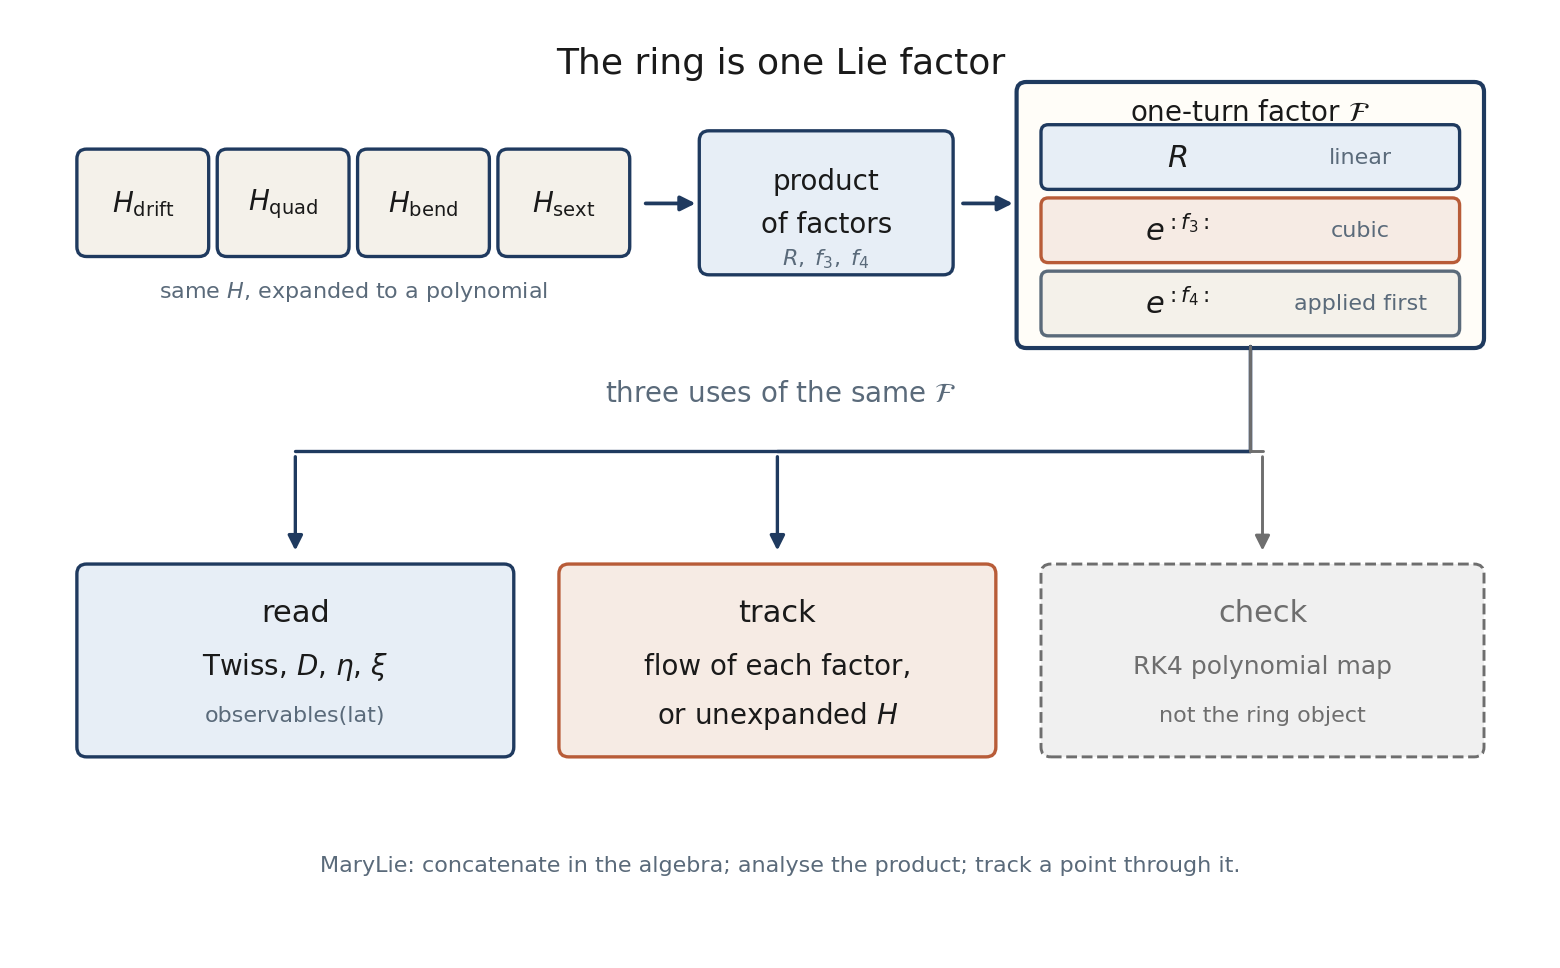
\includegraphics[width=\linewidth]{../src/assets/architecture_object.png}\caption{The ring is one Lie factor: Hamiltonians are concatenated in the algebra; the product is read, tracked, or checked.}\end{figure}

Linear optics, second-order slip and chromaticity are homogeneous pieces
of the same polynomial, not layers derived from one another.

\begin{figure}[htbp]\centering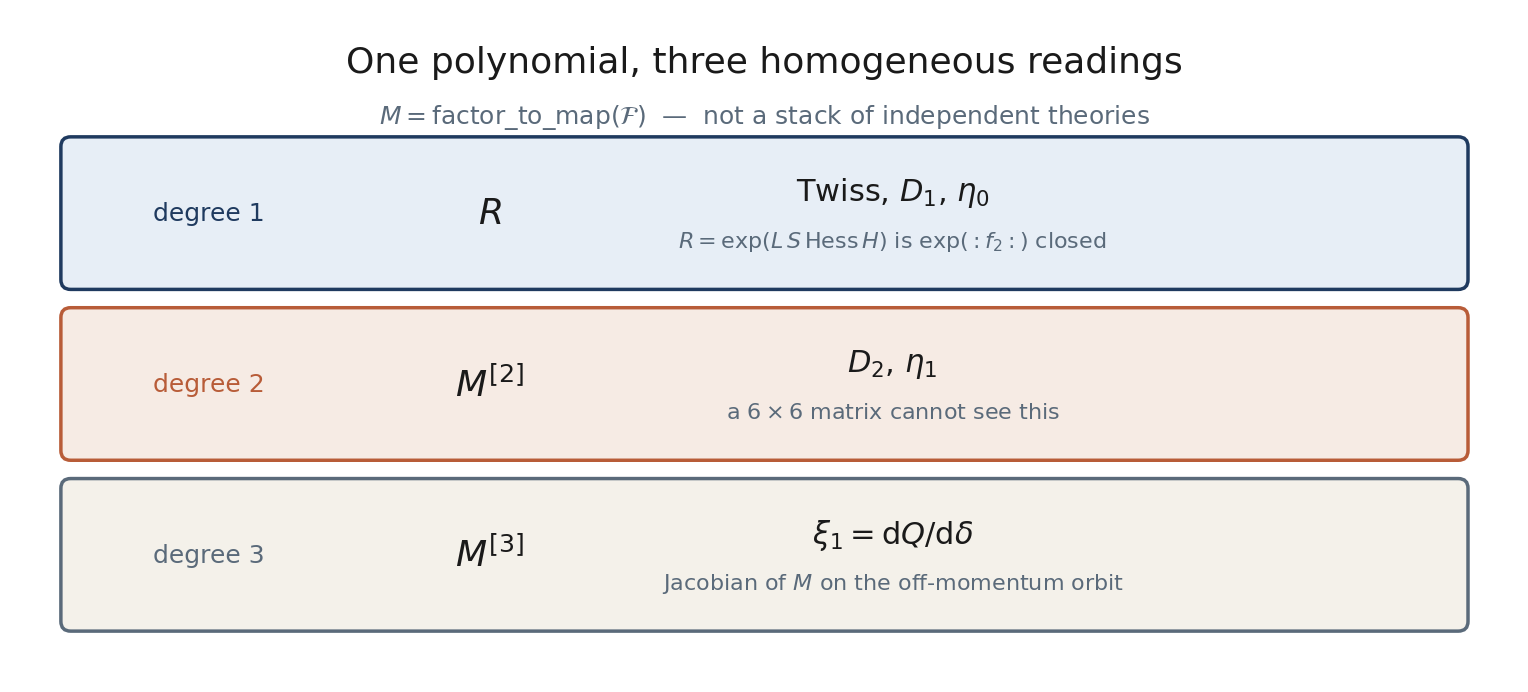
\includegraphics[width=\linewidth]{../src/assets/architecture_orders.png}\caption{One polynomial, three homogeneous readings: degree 1 gives Twiss and $\eta_0$; degree 2 gives $D_2$ and $\eta_1$; degree 3 gives $\xi_1$.}\end{figure}

Contents:

\begin{enumerate}
\item Canonical phase space
\item Element Hamiltonians
\item Lie product of the ring
\item Linear optics
\item Second-order dispersion and momentum compaction
\item Chromaticity
\item Finite-length RF cavity
\item Acceleration and adiabatic damping
\item Longitudinal motion from the ring average
\item Sextupole families
\item Equilibrium momentum shift
\item Assumptions
\end{enumerate}

Figures use the Nuclotron-based lattice at deuteron kinetic energy 270 MeV
unless a ramp from 10 MeV is shown. A separate *Programmer Manual* documents
the implementation.

\clearpage
\section{Canonical phase space}

\subsection{Variables}

The dynamical state at arc length $s$ is the six-vector

\[
z=(x,\,p_x,\,y,\,p_y,\,l,\,\delta).
\]

- $x,y$: transverse displacements from the reference orbit [m].
- $p_x=P_x/p_0$, $p_y=P_y/p_0$: canonical momenta normalised to the
  reference momentum $p_0$.
- $\delta=(p-p_0)/p_0$: relative *momentum* deviation.
- $l=-v(\delta)\,\Delta t$: longitudinal coordinate conjugate to $\delta$,
  with $\Delta t=t-t_0(s)$ the time lag relative to the reference particle
  and $v(\delta)$ the particle speed,

\[
\frac{v(\delta)}{v_0}=\frac{1+\delta}{\beta_0\sqrt{(1+\delta)^2+1/(\beta_0\gamma_0)^2}}.
\]

The reference particle has charge $Ze$, rest energy $mc^2$, Lorentz factor
$\gamma_0$, velocity $v_0=\beta_0 c$ and momentum $p_0$.

\subsection{From $(t,-E)$ to $(l,\delta)$}

The $s$-Hamiltonian is first written with the longitudinal pair
$(t,-E)$. A type-2 generating function at fixed $s$,

\[
F_2(t,\delta;s)=-(t-s/v_0)\,E(\delta)/p_0,
\]

produces the new coordinate $l=\partial F_2/\partial\delta=-(t-s/v_0)\,v(\delta)$
and adds $\partial F_2/\partial s=E(\delta)/(p_0 v_0)$ to the Hamiltonian.
After dropping a constant, that addition is the energy term $e(\delta)$
below. Because $l$ is conjugate to $\delta$, the momentum deviation
$\delta=(p-p_0)/p_0$ is the true relative momentum, not an energy offset.

The symplectic form on this space is the standard one,

\[
\omega=\mathrm{d}x\wedge\mathrm{d}p_x+\mathrm{d}y\wedge\mathrm{d}p_y+\mathrm{d}l\wedge\mathrm{d}\delta,
\]

or in matrix form $S=\mathrm{diag}(S_2,S_2,S_2)$ with
$S_2=\begin{pmatrix}0&1\\-1&0\end{pmatrix}$. A map $z\mapsto\mathcal{M}(z)$
is symplectic iff its Jacobian satisfies $J^\mathsf{T}SJ=S$.

\subsection{Output (non-canonical) coordinates}

For plots and comparison with laboratory data one uses

\[
u=(x,\,x',\,y,\,y',\,\phi,\,\delta),\qquad
x'=\frac{p_x}{p_s},\quad
p_s=\sqrt{(1+\delta)^2-p_x^2-p_y^2},\quad
\phi=-h\omega_0\Delta t=\frac{2\pi h}{C}\,\frac{l}{v(\delta)/v_0}.
\]

$\phi>0$ means early arrival. The set $u$ is \textbf{not} canonical:
$x'$ depends on $\delta$ and $p_y$, and $\phi$ is scaled by
$1/v(\delta)$. Symplecticity is therefore checked only in $z$. The
conversion $z\leftrightarrow u$ is exact (nonlinear); truncated polynomial
maps apply it as a full Taylor polynomial to the map order.

\subsection{Energy term}

Every magnetic Hamiltonian uses

\[
e(\delta)=\frac{1}{\beta_0}\sqrt{(1+\delta)^2+\frac{1}{\beta_0^2\gamma_0^2}}-\frac{1}{\beta_0^2},
\]

chosen so that the irrelevant constant vanishes at $\delta=0$ after removal
of the constant term of $H$.
\clearpage
\section{Element Hamiltonians}

With $p_s=\sqrt{(1+\delta)^2-p_x^2-p_y^2}$, curvature $h=1/\rho$ and
normalised multipoles $k_1=B'/(B\rho)$, $k_2=B''/(B\rho)$, the
$s$-Hamiltonians (hard-edge, no fringe fields) are

\begin{center}\small\begin{tabular}{p{0.475\linewidth}p{0.475\linewidth}}\hline
\textbf{element} & \textbf{$H(z)$}\\\hline
Drift & $e(\delta)-p_s$\\
Quadrupole & $e(\delta)-p_s+\tfrac{k_1}{2}(x^2-y^2)$\\
Sextupole & $e(\delta)-p_s+\tfrac{k_2}{6}(x^3-3xy^2)$\\
Sector bend & $e(\delta)-(1+hx)p_s+hx+\tfrac12 h^2 x^2+\tfrac{k_1}{2}(x^2-y^2)$\\
Marker & $0$\\
Finite RF cavity & $e(\delta)-p_s+A\cos\Phi(l,\delta,s)$ (see Finite-length RF cavity)\\
\hline\end{tabular}\end{center}

For the bend, $\partial H/\partial x|_{z=0}=0$: the reference arc is a
solution of Hamilton's equations.

The bend potential is cut at $hx+\tfrac12 h^2 x^2$. There are no fringe
fields. A gradient in a bend uses the straight-magnet term; curvature
corrections of order $h k_1 x^3$ are omitted (the lattice used here has
$k_1=0$ in every bend).

The Hamiltonian of each magnet is replaced by its Taylor polynomial of
total degree 4 (square root and energy expanded). That polynomial is the
generator. It is not yet a map.

\subsection{Maps from a Hamiltonian}

An $s$-independent Hamiltonian over length $L$ generates the Lie
transformation $\exp(-L:H:)$, with

\[
:f:g=[f,g]=\sum_i\Bigl(\partial_{q_i}f\,\partial_{p_i}g-\partial_{p_i}f\,\partial_{q_i}g\Bigr).
\]

How the ring is assembled from these transformations is in
Lie product of the ring.
\clearpage
\section{Lie product of the ring}

The object of the ring is a product of Lie transformations. A generator is a
polynomial in the canonical coordinates. The Poisson bracket acts on its
coefficients. Substituting truncated maps into one another is a check, not
the definition of the one-turn map. The figures in the home page
show the product, its three uses, and the homogeneous readings of its
polynomial.

\subsection{From a Hamiltonian to a factor}

Hamilton's equations are $\mathrm{d}z/\mathrm{d}s=[z,H]=-:H:z$. Over a
length $L$ with $H$ independent of $s$ the map is the Lie series
$\exp(-L:H:)$. The series is cut at total degree 3 in $z$. The result is
written as a Dragt–Finn factor

\[
\mathcal{M}=R\circ e^{:f_3:}\circ e^{:f_4:}.
\]

Applied to a point, this means: first the time-1 flow of $f_4$, then of
$f_3$, then the linear matrix $R$. Each nonlinear flow is a canonical
transformation for any generator. Tracking integrates those flows by the
implicit midpoint rule, so each factor is symplectic to round-off at any
amplitude.

The polynomial expansion of the same factor is symplectic only up to the
dropped degree.

\subsection{Product of two factors}

Two factors are multiplied in the algebra, not by substituting maps. If
$\mathcal{M}_a$ is applied first and $\mathcal{M}_b$ second,

\[
R=R_b R_a,\qquad
f_3=f_{3a}+f_{3b}\circ R_a,\qquad
f_4=f_{4a}+f_{4b}\circ R_a-\tfrac12[f_{3b}\circ R_a,\,f_{3a}].
\]

The Poisson bracket of two cubics is quartic. Nested brackets are degree 5
and are dropped. The minus in front of the bracket is the BCH term for the
coordinate maps $z\mapsto\exp(:f:)z$; it is fixed by comparing the product
of two elements with the Lie series of that pair.

The one-turn magnetic factor is this product over the lattice.

\subsection{Thin RF kick}

A thin cavity at $\varphi_s=\pi$ is a canonical transformation that fixes
the origin: energy changes at fixed arrival time, then $\delta$ and $l$
are recomputed. It enters the one-turn product as one more Dragt–Finn
factor. The sine of the kick is expanded to the same degree as the magnetic
generators. The exact sine is kept only in the independent integrator of the
unexpanded Hamiltonian.

A cavity with a net energy gain per turn shifts the origin. The product
above is written for maps that fix the origin, so a ramp or a finite cavity
with a closed-orbit offset is a separate problem.

\subsection{Normal form}

The linear part $R$ of the one-turn factor is put into three rotations by
a symplectic matrix $A$, $A^\mathsf{T}SA=S$. The generators in the
normal coordinates $w=A^{-1}z$ are the pull-backs $f(Aw)$.

A rotation acts on a complex monomial
$h_{\mathbf{j}\mathbf{n}}=\prod_k(q_k+ip_k)^{j_k}(q_k-ip_k)^{n_k}$ by the
phase $e^{-i(\mathbf{j}-\mathbf{n})\cdot\boldsymbol{\mu}}$. The homological
operator on a generator is therefore the divisor

\[
F-F\circ r(\mu),\qquad
F_{\mathbf{j}\mathbf{n}}=\frac{-f_{\mathbf{j}\mathbf{n}}}{1-e^{-i(\mathbf{j}-\mathbf{n})\cdot\boldsymbol{\mu}}}.
\]

At degree 3, $\mathbf{j}=\mathbf{n}$ is impossible, so in the absence of
a third-order resonance the whole cubic generator is removed. At degree 4
the kernel is the span of products of actions; those terms stay as the
normal-form Hamiltonian $h_4=\sum_{i\le j}c_{ij}J_i J_j$. The cubic
conjugation contributes $\tfrac12[f_3,F_3]$ to the quartic generator
before this step.

The homological operator is applied to the generators. Conjugation of a
full polynomial map is not used to build the normal form.

\subsection{The torus}

After the normal form there are three amplitudes $J_x,J_y,J_s$ and three
phases $\theta_x,\theta_y,\theta_s$. The torus of those actions is the set
of all triples of phases at those fixed amplitudes: three circles, not a
trajectory and not a list of turns.

One turn adds constant angles to the phases and does not change the
amplitudes. Laboratory $\delta$ is a function of the three phases. The
equilibrium momentum is the average of that function over the whole torus
at once. Pieces odd in the phases average to zero. What remains is linear
in the actions,

\[
\delta_{\mathrm{eq}}=\delta^\ast+d_x J_x+d_y J_y+d_s J_s.
\]

For thin RF on the stationary separatrix, $\delta^\ast$ is a numerical
zero. The cubic-RF correction in $\hat\varphi^2$ is degree $J^2$ and is
not kept.

A long tracking average equals this torus average when the tunes are
incommensurate. Tracking does not build the torus.

\subsection{Independent checks}

Two constructions are not the one-turn Lie product.

\begin{enumerate}
\item Hamilton's equations integrated in the truncated polynomial algebra
\end{enumerate}
   (a differential-algebra map) and composed by substitution. The
   coefficient-wise difference with the expanded Lie product is a
   truncation and step-size error. It is printed; it is not substituted
   into $\delta_{\mathrm{eq}}$.
\begin{enumerate}
\item The unexpanded Hamiltonian (the square root is not a polynomial)
\end{enumerate}
   integrated by a symplectic step, with an exact thin energy kick at the
   end of the turn. This is the amplitude-exact tracking standard.

\clearpage
\section{Linear optics}

The linear map of an element is the closed form of the quadratic Lie
transformation $\exp(:f_2:)$. With
$\mathcal{H}_{ij}=\partial^2 H/\partial z_i\partial z_j|_0$,

\[
R=\exp(L\,S\,\mathcal{H}).
\]

This is not a textbook transport matrix: the Hessian comes from the same
$H$ that generates the nonlinear factor. For plots along $s$ the
matrices are multiplied element by element. For one-turn optics of the
ring, $\mathtt{observables}$ reads the linear factor $\mathcal{F}.R$
of the Lie product, not a second, independent matrix product.

With $\cos\mu=\tfrac12\mathrm{Tr}M_x$,

\[
\beta=\frac{M_{12}}{\sin\mu},\qquad
\alpha=\frac{M_{11}-M_{22}}{2\sin\mu},
\]

and the closed dispersion solves $(I-M_4)D=M_{\cdot 6}$. Momentum compaction
to first order:

\[
\alpha_0=\frac{1}{\gamma_0^2}-\frac{(l|\delta)_{\mathrm{closed}}}{C}
=\frac1C\oint h\,D\,\mathrm{d}s.
\]

Twiss and dispersion propagated in slices close after one turn to machine
precision.

\begin{figure}[htbp]\centering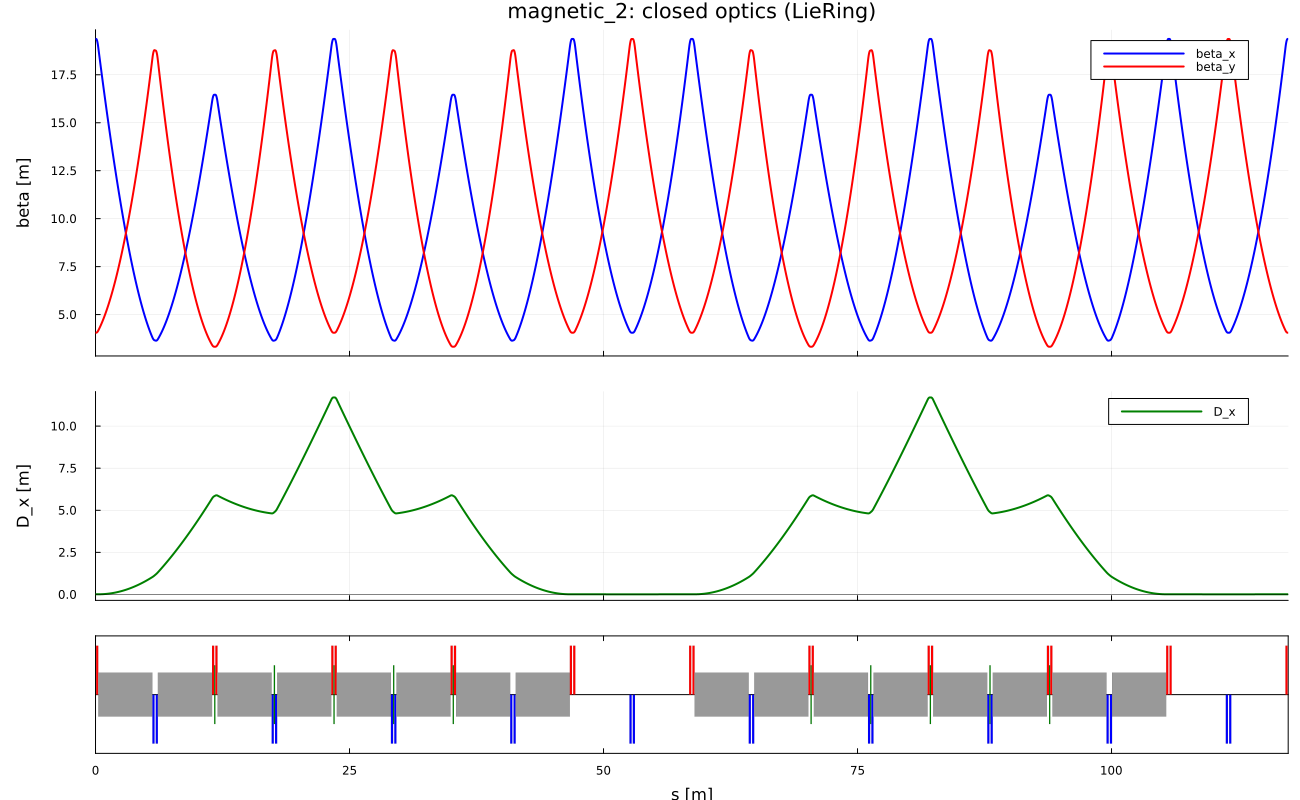
\includegraphics[width=\linewidth]{../src/assets/magnetic_2_twiss.png}\caption{Closed beta functions, horizontal dispersion and magnet layout.}\end{figure}
\clearpage
\section{Second-order dispersion and momentum compaction}

The quadratic piece of the one-turn polynomial. A linear matrix cannot
see $D_2$ or $\eta_1$. Both are read from the same Lie product as
Twiss; they are not a second optical theory.

\subsection{Closed orbit in $\delta$}

\[
z_\perp(\delta)=D_1\delta+D_2\delta^2+O(\delta^3),
\]

from $M_\perp(z_\perp(\delta),\delta)=z_\perp(\delta)$ order by order.

\subsection{Path length and $\alpha_i$}

On the closed orbit the geometric circumference admits the expansion

\[
\frac{C(\delta)}{C_0}=1+\alpha_0\delta+\alpha_1\delta^2+\alpha_2\delta^3+\cdots.
\]

With the canonical coordinate $l$ related to time of flight by
$l=-v\Delta t$, one turn gives
$\Delta l=-C(\delta)+C_0\,v(\delta)/v_0$, hence

\[
\alpha_0=-\frac{l_1}{C}+\frac{1}{\gamma_0^2},\qquad
\alpha_1=-\frac{l_2}{C}+c_2,\qquad
\alpha_2=-\frac{l_3}{C}+c_3,
\]

where $v/v_0-1=c_1\delta+c_2\delta^2+c_3\delta^3$ and
$c_1=1/\gamma_0^2$. Equivalently, $\alpha_i$ may be fitted from
$C(\delta)/C_0$ evaluated on closed orbits at several $\delta$.

\subsection{Slip factor}

The relative change of revolution period is the time of flight of one turn.
With $l=-v\Delta t$ one has $\Delta T/T_0=-(l/C)/(v/v_0)$, so on the
closed orbit

\[
\eta_0=-\frac{l_1}{C}=\alpha_0-\frac{1}{\gamma_0^2},\qquad
\eta_1=-\frac{l_2}{C}+\frac{l_1}{C}\,\frac{1}{\gamma_0^2}
=\alpha_1-\frac{\alpha_0}{\gamma_0^2}+\frac{3\beta_0^2}{2\gamma_0^2}+\frac{1}{\gamma_0^4}.
\]

These are the coefficients used in the averaged longitudinal Hamiltonian
and in the formula for $\delta_{\mathrm{eq}}$. They come from the
one-turn Lie product, expanded to a polynomial only to read $l_1$ and
$l_2$.

\begin{figure}[htbp]\centering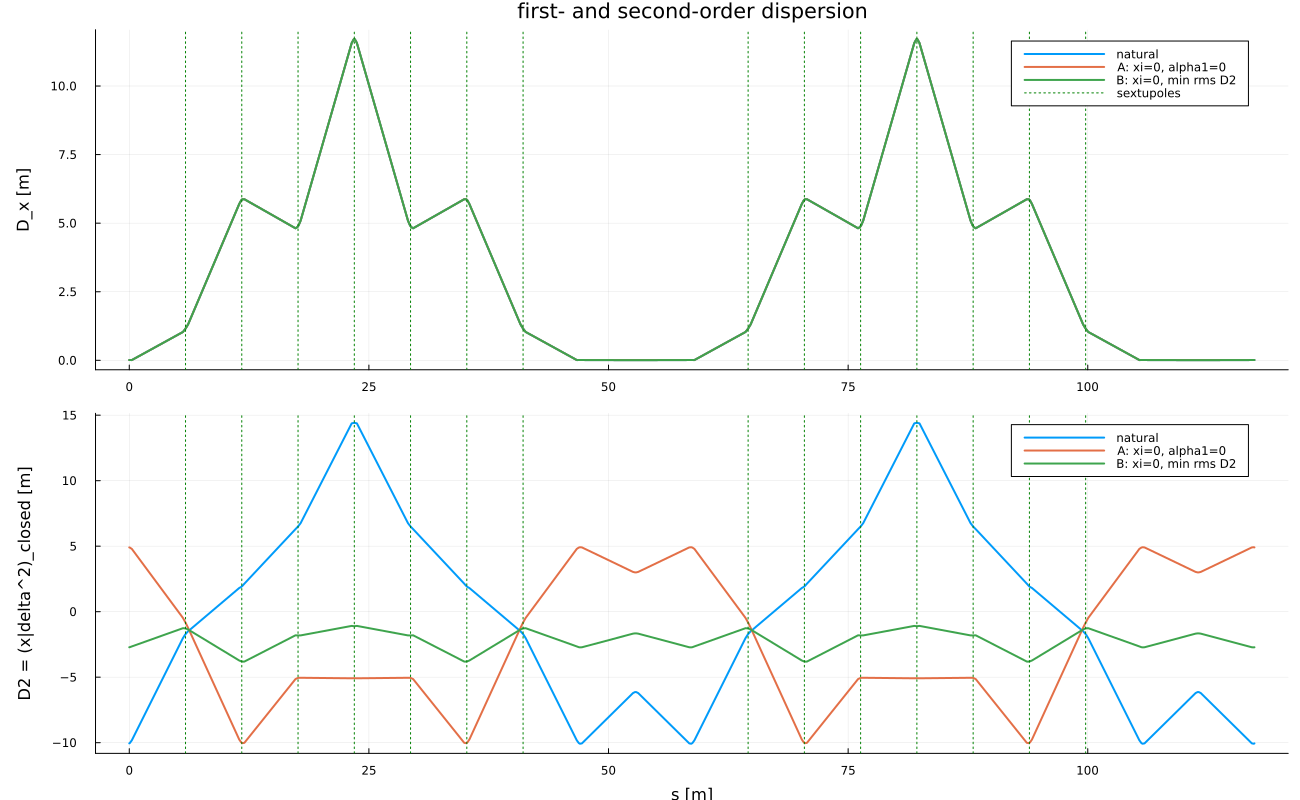
\includegraphics[width=\linewidth]{../src/assets/sextupoles_dispersion2.png}\caption{Second-order dispersion along the ring.}\end{figure}
\clearpage
\section{Chromaticity}

Chromaticity is a reading of the one-turn polynomial, not a descendant of
the Twiss functions. At fixed $\delta$ the transverse motion about
$z_\perp(\delta)$ is linearised. The tunes $Q_{x,y}(\delta)$ from
$\cos 2\pi Q=\tfrac12\mathrm{Tr}J(\delta)$ expand as

\[
Q(\delta)=Q_0+\xi_1\delta+\tfrac12\xi_2\delta^2.
\]

Since $\delta$ is conserved without RF, these are invariants of the
one-turn map. Cross-check: integrate the exact Hamiltonians at several
$\delta$ and fit the tune of a small betatron oscillation.

\begin{figure}[htbp]\centering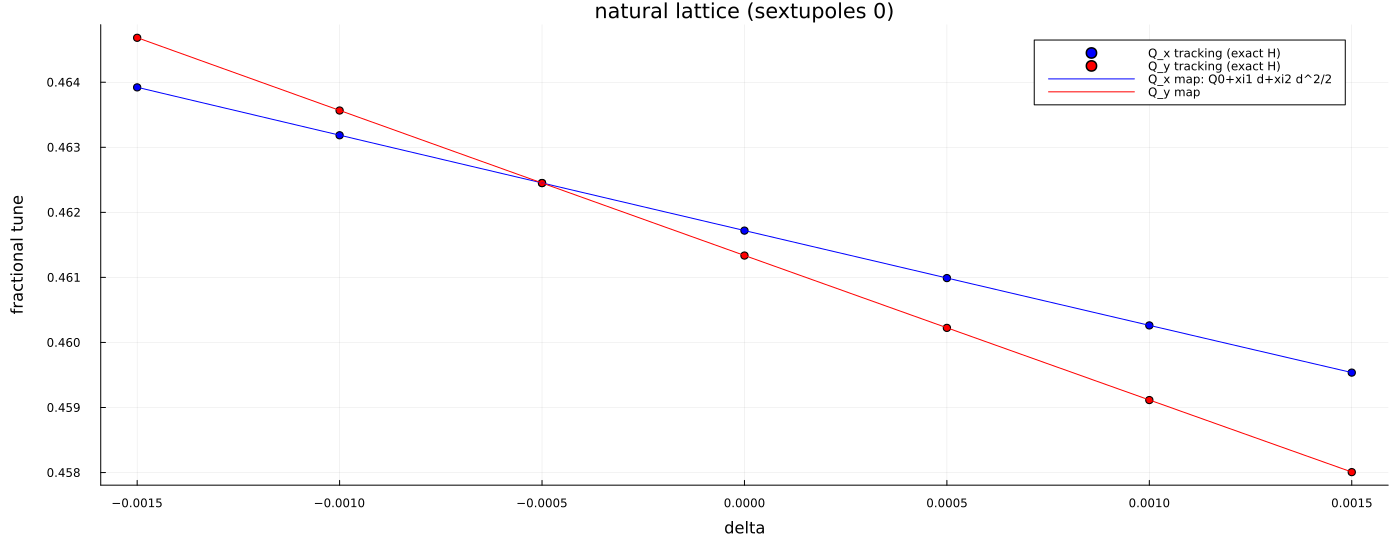
\includegraphics[width=\linewidth]{../src/assets/chromaticity_natural.png}\caption{Fractional tunes versus momentum deviation.}\end{figure}
\clearpage
\section{Fringe fields of dipoles and quadrupoles}

The body Hamiltonian of a magnet assumes a field that switches on and off
abruptly at the magnet ends. A real field rises over a distance of the
order of the gap. The fringe region is described by separate thin maps at
the entrance and the exit of the magnet; the body map is unchanged. The
lattice keeps the physical description of the magnet: length, bending
angle, pole-face angles $e_1, e_2$, full gap $g$ and fringe integral
$K = \mathrm{FINT}$. The edge model is chosen when the ring map is formed.

\subsection{Hard edge, linear order}

For a pole face rotated by $e$ the field boundary is not perpendicular to
the reference orbit. The extra (or missing) triangle of field acts as a thin
lens

\[
\Delta p_x = h\tan e\;x,\qquad \Delta p_y = -h\tan\psi\;y,
\qquad \psi = e - h g K\,\frac{1+\sin^2 e}{\cos e},
\]

with $h = 1/\rho$. The correction $\psi - e$ comes from the finite
extent of the fringe: inside it the orbit already bends, so the angle
between orbit and field boundary changes. For a sector bend with
$e = 0$ and $K = 0$ the linear edge map is the identity.

\subsection{Hard edge, nonlinear}

The vertical kick depends on the angle between the particle trajectory and
the field boundary, not on the angle of the reference orbit. With the slope
$x' = p_x/p_s$, $p_s = \sqrt{(1+\delta)^2-p_x^2-p_y^2}$, the effective
angle is $e + x'$ at the entrance and $e - x'$ at the exit. The edge is
the Lie transformation $\exp(-:K:)$ with the generator

\[
K_{\rm in} = -\frac{h\tan e}{2}\,x^2 + \frac{h}{2}\,y^2\,\tan\!\left(\psi + \arctan x'\right),
\qquad
K_{\rm out} = -\frac{h\tan e}{2}\,x^2 + \frac{h}{2}\,y^2\,\tan\!\left(\psi - \arctan x'\right).
\]

Because the edge is generated by a single polynomial $K$, the map is
symplectic to every order. For $e = 0$ the leading term is
$K = \pm h\,y^2 p_x/(2 p_s)$. On the dispersive orbit $p_x = D'\delta$,
so the vertical focusing of each edge changes linearly with $\delta$: the
edges contribute to the vertical chromaticity even when their linear
effect vanishes. The same term follows from the longitudinal field
$B_s = y\,\partial_s B_y$ of a step profile.

For quadrupoles the leading hard-edge effect is of fourth degree in the
generator,

\[
K = \pm\frac{k_1}{12(1+\delta)}\left(x^3 p_x + 3 x y^2 p_x - 3 x^2 y p_y - y^3 p_y\right),
\]

($+$ entrance, $-$ exit). It changes the amplitude-dependent tune shift
and leaves the tunes and the first-order chromaticity unchanged.

\subsection{Soft edge}

The field on the reference orbit is $B_y = B_0 F(z)$ with a profile
$F$ that rises from 0 outside to 1 inside. The effective field boundary
(EFB) at $z = 0$ is fixed by equal area,

\[
\int_{-W}^{0} F\,dz = \int_{0}^{W} (1-F)\,dz,
\]

so the integrated field and the bending angle are those of the hard-edge
magnet. The fringe integral is $gK = \int F(1-F)\,dz$. Profiles:

\begin{itemize}
\item Enge: $F = 1/\left(1+\exp P(-z/g)\right)$, $P$ a polynomial;
\item hyperbolic tangent: $F = \tfrac12\left(1+\tanh(z/\lambda)\right)$,
\end{itemize}
  $gK = \lambda/2$;
\begin{itemize}
\item linear ramp of width $w$: $gK = w/6$;
\item tabulated profile from a field map, interpolated and normalised.
\end{itemize}

The soft region $[-W, W]$ replaces the last length $W$ of the drift
and the first length $W$ of the body of the hard-edge layout. The total
length and the bending angle are preserved.

\#\#\# Hamiltonian in the fringe

In the Frenet frame of an orbit that follows the local field,
$h(s) = h_0 F(s)$,

\[
H = e(\delta) - (1+hx)\sqrt{(1+\delta)^2 - (p_x - a_x)^2 - p_y^2}
    + h x + \frac{h^2x^2}{2}
    + \frac{b_1}{2}(x^2-y^2) + \frac{b_2}{6}(x^3-3xy^2),
\qquad a_x = -\frac{y^2 h_0 F'(s)}{2(1+hx)} .
\]

The vector potential $a_x$ gives the longitudinal field
$B_s = y\,b'/(1+hx)$ and the second-order vertical dependence
$B_y = b - \tfrac{y^2}{2}\left[b''/(1+hx)^2 - b'h'x/(1+hx)^3\right]$;
together they satisfy $\nabla\times B = 0$ to second order in $y$.

The field boundary is a straight line perpendicular to the field-free
orbit, while the frame follows the curved orbit. A point at transverse
position $x$ sees the profile at $z = s + x\,\theta(s)$, where
$\theta$ is the angle between the local orbit and the field-free orbit,
$\theta = h_0\int_{-W}^{s}F$ at the entrance and
$\theta = -h_0\int_{s}^{W}F$ at the exit. Expansion in $x$ gives the
gradient $b_1 = h_0F'\theta$ and the sextupole-like term
$b_2 = h_0F''\theta^2$. The integrated gradient is

\[
\int b_1\,ds = h_0^2\int F(1-F)\,dz = h_0^2\,gK ,
\]

which is the vertical focusing of the $\psi$ correction above; in the
horizontal plane it cancels the weak-focusing deficit
$h_0^2\int (F^2-\Theta)\,dz = -h_0^2 gK$ of the shortened field. A soft
edge therefore reproduces the linear hard-edge model with the fringe
integral of its profile, and its nonlinear terms tend to the nonlinear
hard edge as $g\to 0$.

\#\#\# Integration through the fringe

The Hamiltonian depends on $s$. Three methods give the map of the
region:

\begin{itemize}
\item \textbf{Splitting}: $n$ slices with $F, F', F''$ replaced by slice values;
\end{itemize}
  each slice is $\exp(-\Delta s :H_k:)$. Second order with one step per
  slice, fourth order with the Yoshida composition
  $w_1 = 1/(2-2^{1/3})$, $w_0 = 1-2w_1$. Every slice is a Lie
  transformation, so the map is symplectic.
\begin{itemize}
\item \textbf{Magnus expansion}: on each sub-interval $\exp(-:\Omega:)$ with
\end{itemize}
  $\Omega = \Delta s\,H(s_m)$ (second order) or, with two Gauss nodes,
  the fourth-order form below. Symplectic.
\begin{itemize}
\item \textbf{Taylor integration}: the equations of motion integrated in truncated
\end{itemize}
  power series (differential algebra) with step halving until the map
  changes by less than a tolerance. Not symplectic by construction; the
  defect is of the order of the tolerance.

Fourth-order Magnus step ($H_1, H_2$ at the Gauss nodes
$s_m \mp \Delta s\sqrt3/6$, $H_1$ first):

\[
\Omega = \frac{\Delta s}{2}(H_1+H_2) - \frac{\sqrt3}{12}\Delta s^2\,[H_1,H_2] .
\]

For profiles with kinks (linear ramp, tabulated data) the derivatives are
taken as averages over the slice or step, which keeps $\int F'$ and
$\int F''$ exact.

\subsection{Validation}

\begin{itemize}
\item No edge: the ring map is identical to the plain lattice.
\item $g\to 0$: the soft-edge tunes and chromaticities approach the
\end{itemize}
  nonlinear hard edge linearly in $g$.
\begin{itemize}
\item Linear focusing of a soft edge equals that of a hard edge with
\end{itemize}
  $K = \int F(1-F)dz/g$.
\begin{itemize}
\item Different methods and profiles with the same fringe integral agree to the
\end{itemize}
  accuracy of the slicing.
\begin{itemize}
\item $J^{\mathsf T} S J = S$ for the edge maps to round-off (Lie methods).
\end{itemize}

\subsection{Approximations}

\begin{itemize}
\item The fringe region is treated as straight in the gradient term
\end{itemize}
  $b_1, b_2$; corrections of order $h_0^2 g^2$ are not included.
\begin{itemize}
\item The displacement between the soft-edge and hard-edge reference orbits
\end{itemize}
  (of order $h_0 g^2$) is absorbed in the frames; only maps about the
  reference are formed.
\begin{itemize}
\item Pole-face rotation in a soft edge is the linear wedge at the EFB; the
\end{itemize}
  dependence of the profile on $x\tan e$ is not expanded further.
\begin{itemize}
\item Fields are expanded to second order in $y$; quadrupole soft edges are
\end{itemize}
  not modelled.

\clearpage
\section{Finite-length RF cavity}

The cavity of length $L$ carries a purely longitudinal on-axis field.
With $q A_s/p_0=-A\cos(\omega t+\psi)$ and $t=s/v_0-l/v(\delta)$,

\[
H_{\mathrm{cav}}=e(\delta)-p_s+A\cos\Phi,\qquad
\Phi=\frac{\omega(s-L/2)}{v_0}-\frac{\omega\,l}{v(\delta)}-\phi_s,
\]

\[
A=\frac{ZV}{p_0 c}\,\frac{c}{\omega L},\qquad \omega=h\omega_0=\frac{2\pi h v_0}{C}.
\]

Hamilton's equation $\mathrm{d}\delta/\mathrm{d}s=-\partial H/\partial l$
is equivalent to $\mathrm{d}E/\mathrm{d}s=-(ZV/L)\sin\Phi$. Integrated over
the cavity the energy gain is

\[
\Delta E=ZVT\sin(\phi_s+\phi),\qquad
T=\frac{\sin(\theta/2)}{\theta/2},\quad \theta=\frac{2\pi h L}{C}.
\]

$H_{\mathrm{cav}}$ depends on $s$; it is integrated by a symplectic
$s$-dependent scheme (implicit midpoint, Yoshida 4th order). Transverse RF
fields are omitted. The thin-kick limit $L\to 0$ recovers an instantaneous
energy change $ZV\sin(\phi_s+\phi)$ at fixed $(x,p_x,y,p_y,l)$.
\clearpage
\section{Acceleration and adiabatic damping}

After the cavity the synchronous particle has $\delta_s\neq 0$. It is made
the new reference:

\[
p_0'=p_0(1+\delta_s),\quad
1+\delta'=\frac{1+\delta}{1+\delta_s},\quad
p_x'=\frac{p_x}{1+\delta_s},\quad
p_y'=\frac{p_y}{1+\delta_s},\quad
\Delta t'=\Delta t-\Delta t_s.
\]

Positions are unchanged. Magnets are assumed to ramp with $p_0$ (normalised
strengths fixed); the RF frequency follows $h\omega_0(p_0)$.

The physical transverse momentum $P_x=p_0 p_x$ is invariant under a
longitudinal field, so $p_x\propto 1/p_0$. The Courant–Snyder action in
normalised variables then scales as $J\propto 1/p_0$, and betatron
amplitudes damp as

\[
\frac{A(n)}{A(0)}=\sqrt{\frac{p_{\mathrm{inj}}}{p_0(n)}}.
\]

\begin{figure}[htbp]\centering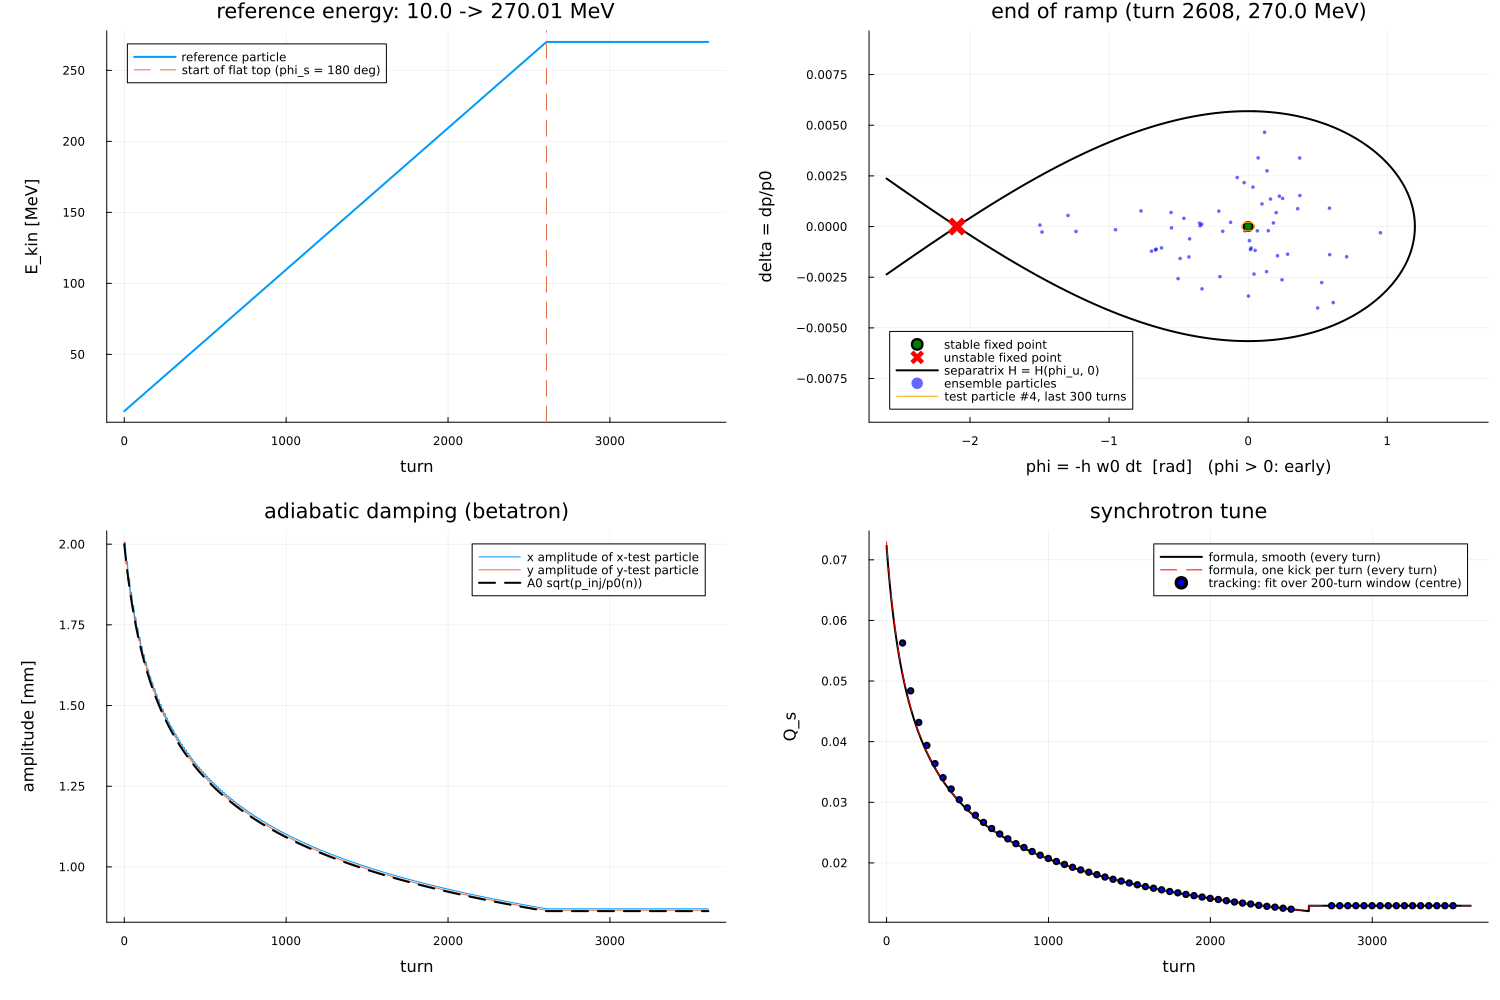
\includegraphics[width=\linewidth]{../src/assets/acceleration.png}\caption{Reference energy, longitudinal phase space with separatrix, adiabatic damping of betatron amplitudes, and synchrotron tune during a ramp.}\end{figure}
\clearpage
\section{Longitudinal motion from the ring average}

\subsection{From the 6D Hamiltonian to a 2D synchrotron Hamiltonian}

Over one turn the magnetic lattice advances $(l,\delta)$ through the
element Hamiltonians. The slip coefficients $\eta_0,\eta_1$ are those of
the time of flight. A thin RF kick changes $\delta$ at fixed arrival time.
Coarse-graining to one map per turn in the variables
$(\phi,\delta)$ with $\phi=-h\omega_0\Delta t$ gives

\[
\begin{aligned}
\phi_{n+1}&=\phi_n-2\pi h\bigl(\eta_0\delta_{n+1}+\eta_1\delta_{n+1}^2+\cdots\bigr),\\
\delta_{n+1}&=\delta_n+A\bigl(\sin(\phi_s+\phi_n)-\sin\phi_s\bigr),\qquad
A=\frac{ZVT}{\beta_0^2 E_0}.
\end{aligned}
\]

Treating the turn number as continuous yields the smooth Hamiltonian

\[
H(\phi,\delta)=-2\pi h\Bigl(\frac{\eta_0\delta^2}{2}+\frac{\eta_1\delta^3}{3}\Bigr)
+A\bigl(\cos(\phi_s+\phi)+\phi\sin\phi_s\bigr),
\]

which is the average of the full 6D dynamics over one revolution under the
assumptions of a single RF station, no transverse–longitudinal coupling in the
averaged equations, and $\delta$ small enough that the closed-orbit expansion
of the path length converges. Fixed points on $\delta=0$: stable $\phi=0$,
unstable $\phi_u=\pi-2\phi_s$. The \textbf{separatrix} is the level set
$H=H(\phi_u,0)$; the RF bucket is the region around the origin inside it.
Stability requires $\eta_0\cos\phi_s>0$.

Small-amplitude synchrotron tune:

\[
Q_s=\sqrt{\frac{h\,\eta_0\,ZVT\cos\phi_s}{2\pi\beta_0^2 E_0}}
\qquad\text{(smooth)},\qquad
\cos(2\pi Q_s^{\mathrm{kick}})=1-\tfrac12(2\pi Q_s)^2
\qquad\text{(one kick/turn)}.
\]

\subsection{Element-by-element view of one turn}

Left: absolute $(\phi,\delta)$ with the analytic separatrix. Right: change
relative to the turn start, with fixed axes set by lattice/RF scales —

- horizontal: $\pm 1.5\,|2\pi h\eta_0|\,\delta_{\mathrm{ens}}$ (full-turn
  phase-slip scale for the largest $|\delta|$ in the ensemble);
- vertical: $\pm 1.5\,A$ (RF kick amplitude).

Only the cavity changes $\delta$ within a turn; $\phi$ changes continuously
through path length and velocity.

\begin{quote}\emph{Animation (see HTML or GIF file): Ensemble during acceleration (left: absolute; right: $\delta$ in units of the current bucket half-height).}\end{quote}

\begin{quote}\emph{Animation (see HTML or GIF file): One turn element by element (left: absolute with separatrix; right: intra-turn change on fixed physical axes).}\end{quote}
\clearpage
\section{Sextupole families}

A thin sextupole of integrated strength $k_2 L$ contributes to first-order
chromaticity

\[
\Delta\xi_{x,y}=\pm\frac{1}{4\pi}\sum k_2 L\,\beta_{x,y}D
\]

and to second-order dispersion / $\alpha_1$ through terms $\propto k_2 L D^2$.
Three families placed at maxima of $D_x$, $\beta_x$ and $\beta_y$ therefore
control $(\xi_x,\xi_y,\alpha_1,D_2)$ nearly independently. Strengths may be
chosen to null $\xi_x,\xi_y$ and optionally $\alpha_1$ or rms $D_2$; that
choice is an optimisation problem, not part of the lattice model. The natural
lattice has vanishing sextupole strengths.

\begin{figure}[htbp]\centering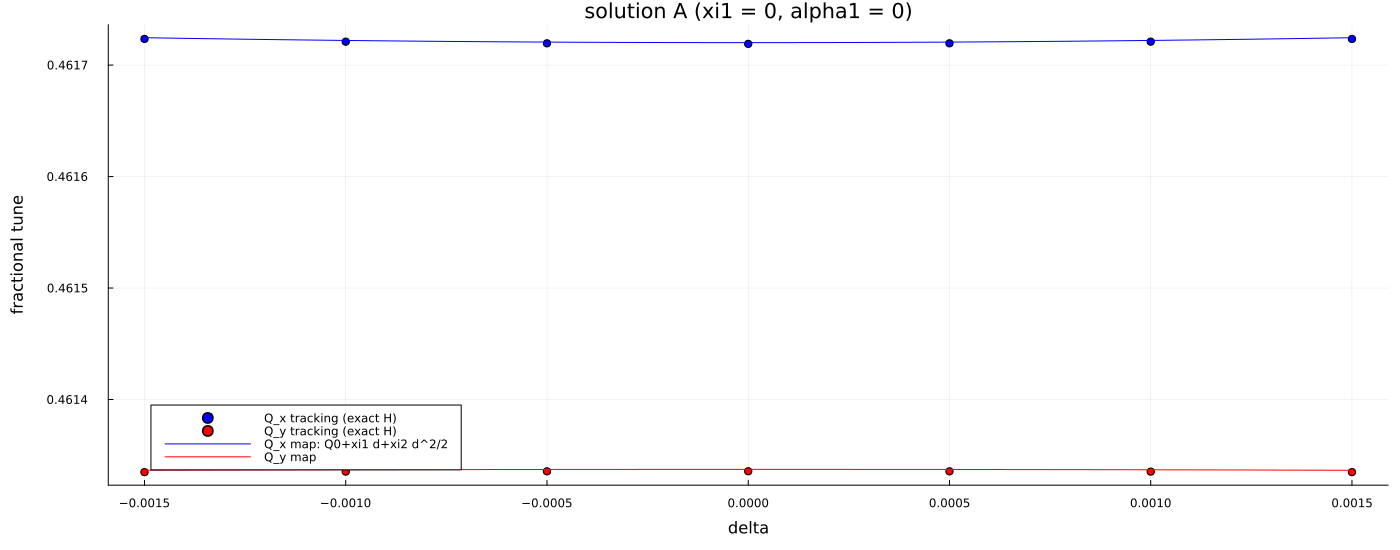
\includegraphics[width=\linewidth]{../src/assets/chromaticity_corrected.png}\caption{Tunes versus $\delta$ after chromaticity correction.}\end{figure}
\clearpage
\section{Equilibrium momentum shift}

A particle that oscillates in a stationary RF bucket ($\varphi_s=\pi$,
below transition) does not have mean relative momentum zero. The RF phase
returns to itself after a synchrotron period only if the mean time of flight
matches the RF period. With a nonlinear slip factor that condition fixes a
nonzero mean

\[
\delta_{\mathrm{eq}}
=-\frac{\eta_1\langle\delta^2\rangle+\Lambda}{\eta_0},\qquad
\Lambda=-\frac{2\pi}{C}\bigl(J_x\xi_x+J_y\xi_y\bigr).
\]

Here $\eta_0,\eta_1$ are the time-of-flight slip coefficients,
$\xi_{x,y}$ the linear chromaticities, and $J_{x,y}$ the Courant–Snyder
actions. For a linear synchrotron oscillation $\langle\delta^2\rangle=\delta_m^2/2$.
A cubic truncation of the RF waveform multiplies the $\eta_1$ piece by
$1-\hat\varphi^2/32$ and shifts the synchrotron frequency by
$\Omega/\omega_s=1-\hat\varphi^2/16$. That correction is second order in
the actions and is not kept in the normal form below.

The RF is a thin energy kick at one point of the ring. A finite-length
cavity has its own closed-orbit offset in $\delta$; that is a separate
study.

\subsection{From the torus}

The one-turn map is the Lie product of the magnetic factors and the thin
kick. After the linear symplectic normalisation and the homological
removal of non-resonant generators, motion is uniform rotation of three
phases at three fixed actions. The torus of those actions is the set of
all triples of phases. Laboratory $\delta$ is a function on that torus.
$\delta_{\mathrm{eq}}$ is the average of $\delta$ over the whole torus:

\[
\delta_{\mathrm{eq}}=\delta^\ast+d_x J_x+d_y J_y+d_s J_s.
\]

For thin RF at $\varphi_s=\pi$, $\delta^\ast=0$. The coefficients $d_k$
are the quadratic part of the sixth component of the normalising
transformation, averaged over angles. They do not use $\eta$ or
$\xi$. Substituting $\delta_m^2=2\sigma_\delta^2 J_s$ into the formula
above reproduces them to relative $10^{-6}$:

\begin{center}\small\begin{tabular}{p{0.238\linewidth}p{0.238\linewidth}p{0.238\linewidth}p{0.238\linewidth}}\hline
\textbf{} & \textbf{$d_x$ [1/m]} & \textbf{$d_y$ [1/m]} & \textbf{$d_s$ [1/m]}\\\hline
torus average & 0.14665244 & 0.22328941 & $2.477064\times 10^{-3}$\\
formula & 0.14665257 & 0.22328971 & $2.477064\times 10^{-3}$\\
\hline\end{tabular}\end{center}

Element-by-element symplectic tracking of the unexpanded Hamiltonians,
with the exact thin kick, gives the same $\delta_{\mathrm{eq}}$ to a
few parts in $10^3$ at $\delta_m\le 10^{-3}$. The residual grows as
$\delta_m^2$ (the next order, not kept). A long time average equals the
torus average when the tunes are incommensurate. The torus itself is not
built from the tracking samples.

The mean energy also receives a kinematic piece from $\langle\delta^2\rangle$:

\[
\Delta E_{\mathrm{eq}}
=\beta_s^2 E_s\Bigl(\delta_{\mathrm{eq}}+\frac{\delta_m^2}{4\gamma_s^2}\Bigr).
\]

\clearpage
\section{Assumptions}

Remaining modelling assumptions (accepted design choices such as injection
energy, RF parameters, CODATA mass, and the interpretation of the lattice
file are recorded in the Programmer Manual, not here).

\begin{enumerate}
\item Hard-edge magnets, no fringe fields.
\item No space charge, impedances, radiation or alignment errors.
\item RF field purely longitudinal on axis (no transverse RF).
\item Magnets and RF frequency scale with the reference momentum during
\end{enumerate}
   acceleration.
\begin{enumerate}
\item Single RF station per turn for the averaged longitudinal Hamiltonian.
\item The one-turn object is the Lie product of Dragt–Finn factors, truncated
\end{enumerate}
   at degree 4 in the generators. Its polynomial expansion is symplectic
   only up to the dropped degree. Integration of the unexpanded
   Hamiltonian is symplectic to round-off.
\begin{enumerate}
\item The product is written for maps that fix the origin (thin RF at
\end{enumerate}
   $\varphi_s=\pi$). A net energy gain per turn is a separate problem.
\end{document}
